\section{Exponential Distribution}
\label{sec:expon-distr}


\subsection*{Theory and Exercises}

\Opensolutionfile{hint}
\Opensolutionfile{ans}

In the previous section we introduced the Poisson process as a natural model of the number of jobs arriving in during intervals of time.  As we will see in the sections to come, the modeling and analysis of any queueing system is typically easier if we specificy  the (probability)
distribution of the interarrival times, i.e., the time between consecutive arrival epochs of jobs.
A particular fruitful model for the distribution of the interarrival times is the exponential distribution. Here we show how this relates to the Poisson distribution,  and we also derive many useful general probability concepts and apply these to the exponential distribution.  Then we use simulation to provide yet further movivation for the use of the exponential distribution as a useful model for interarrival times of customers.

Let us assume that the interarrival times form a sequence $\{X_i\}$ of \recall{independent and identically distributed  (i.i.d.)}  random variables, and let us write $X$ for the generic
random time between two successive arrivals. For many queueing
systems, measurements of the interarrival times between consecutive
arrivals show that it is reasonable to model an interarrival $X$ as
an \recall{exponentially distributed} random variable, i.e.,
\begin{equation*}
  \P{X \leq t} = 1- e^{-\lambda t}
\end{equation*}
Moreover,  the exponential distribution  derives directly from the Poisson distribution. Observe that, if there are no arrivals in some interval $[0,t]$, then it
must be that $N(t) = 0$. Hence, the first interarrival time $X$, i.e., the time until the first customer,  must be larger than $t$.  Therefore,
\begin{equation*}
 \P{X1> t} = \P{N(t) = 0} = e^{-\lambda t} \frac{(\lambda t)^0}{0!}= e^{-\lambda t}.
\end{equation*}
Recall that the constant $\lambda$ is called the arrival
\recall{rate}.  

In the sequel we often write $X\sim \exp(\lambda)$ to
mean that~$X$ is exponentially distributed with rate~$\lambda$.



\begin{exercise} 
In the above expression for $\P{X\leq t}$ we require that $\lambda>0$. What would happen if you would allow $\lambda$ to be zero or negative?
\begin{hint}
  The interpretation of the function $1-e^{-\lambda t}$ is a probability. What are the consequences of this? What happens if $\lambda=0$?
\end{hint}
\begin{solution}
  If $\lambda<0$, then $1-e^{-\lambda t}$ grows to $-\infty$ if $t\to \infty$. Just by itself this is not a problem. However, in our case $1-e^{-\lambda t}$ has the interpretation of a distribution function. Now, recall that a distribution function is bounded to values in the interval $[0,1]$.

Suppose $\lambda=0$. Then $\P{X\leq t} = 1-e^{0} = 0$. In words, this would mean that the probability of a finite interarrival time between any two customers is zero. So, no customers can arrive in this case. 
\end{solution}
\end{exercise}

\begin{exercise} \label{exer:lambda}
  If the random variable $X\sim\exp(\lambda)$, show that its mean $\E X = \frac{1}\lambda$. Interpret this result.
  \begin{hint}
 \begin{equation*}
    \E X = \int_0^\infty t f(t)\, \d t =
    \int_0^\infty t \lambda e^{-\lambda t}\, \d t 
  \end{equation*}
  where~$f(t)=\lambda e^{-\lambda t}$ is the density function of the distribution function $F$ of $X$. Now solve the integral.
  \end{hint}
  \begin{solution}
    \begin{equation*}
      \begin{split}
\E{X} 
&= \int_0^\infty t \lambda e^{-\lambda t} \d t, \quad\text{density is } \lambda e^{-\lambda t} \\
&=   \lambda^{-1} \int_0^\infty u e^{-u}\, \d u, \quad \text{ by  change of variable $u=\lambda t$},   \\
&=  -\lambda^{-1}\left. t e^{- t}\right|_0^\infty + \lambda^{-1} \int_0^\infty e^{- t} \d t\\
&=  - \lambda^{-1} \left. e^{- t} \right|_0^\infty =  \frac1\lambda.
      \end{split}
    \end{equation*}

For the interpretation, if jobs arrive at rate $\lambda$, the average time between two arrivals is $\lambda^{-1}$.
  \end{solution}
\end{exercise}


\begin{exercise} 
  If $X\sim\exp(\lambda)$, show that its second moment $\E{X^2} =  \frac{2}{\lambda^2}$.
  \begin{hint}
  \begin{equation*}
  \E{X^2}= \int_0^\infty t^2 \lambda e^{-\lambda t}\, \d t =  \frac{2}{\lambda^2}.
  \end{equation*}
  \end{hint}
  \begin{solution}
    \begin{equation*}
      \begin{split}
\E{X^2} 
&= \int_0^\infty t^2 \lambda e^{-\lambda t} \d t \\
&=   \lambda^{-2} \int_0^\infty u^2 e^{-u}\, \d u, \quad \text{ by  change of variable $u=\lambda t$},   \\
&= -\lambda^{-2}\left. t^2 e^{- t}\right|_0^\infty + 2\lambda^{-2}\int_0^\infty t e^{- t} \d t \\
&=  -2\lambda^{-2}\left. t e^{- t}\right|_0^\infty + 2\lambda^{-2} \int_0^\infty e^{- t} \d t\\
&=  - 2\lambda^{-2} \left. e^{- t} \right|_0^\infty \\
&=  2/\lambda^2.
      \end{split}
    \end{equation*}
  \end{solution}
\end{exercise}

\begin{exercise} 
  If $X\sim\exp(\lambda)$, show that the \recall{variance}
$\V X = \lambda^{-2}$.
  \begin{hint} Use, and memorize, the very practical formula
  \begin{equation*}
  \V X = \E X^2 - (\E X)^2.
  \end{equation*}
  \end{hint}
  \begin{solution}
    By the previous problems, $\E{X^2}=2/\lambda^2$ and $\E X = \lambda$. 
  \end{solution}
\end{exercise}

The  above exercises can also be easily solved with the moment generating function of $X\geq 0$
\begin{equation*}
  M_X(t) = \E{e^{tX}} = \int_0^\infty e^{tx} \lambda e^{-\lambda x} \d x.
\end{equation*}

\begin{exercise}
Why do we require that $t \in [0, \lambda)$ in the definition of $M_X(t)$?
\begin{solution}
\begin{equation*}
  M_X(t) = \E{e^{tX}} = \lambda \int_0^\infty e^{-(\lambda-t) x}\d x.
\end{equation*}
  If $t - \lambda>0$, then this integral becomes $\infty$. 
\end{solution}
\end{exercise}

\begin{exercise}
  What is $M_x(0)?$
  \begin{solution}
    $M_X(0) = \E{e^{0 X}} = \E{e^0} = \E{1} = 1$
  \end{solution}
\end{exercise}

\begin{exercise}\label{ex:33}
 If $X$ is an exponentially distributed random variable with
    parameter $\lambda$, show that its moment generating function
    \begin{equation*}
    M_X(t) = \frac{\lambda}{\lambda-t}.
    \end{equation*}
   \begin{hint}
    \begin{equation*}
      M_X(t) = \E{\exp(t X)} =\int_0^\infty e^{tx} f(x) \,\d x.
\end{equation*}
\end{hint}
    \begin{solution}
    \begin{equation*}
      \begin{split}
      M_X(t) &= \E{\exp(t X)} = 
=\int_0^\infty e^{tx} f(x) \,\d x 
=\int_0^\infty e^{tx} \lambda e^{-\lambda x} \,\d x  \\
&=\lambda \int_0^\infty e^{(t-\lambda)x} \,\d x 
=\frac{\lambda}{\lambda -t}.
      \end{split}
    \end{equation*}
    \end{solution}
  \end{exercise}

\begin{exercise}
    Use the moment generating function to show that 
    \begin{align*}
      \E{X} &=\frac1\lambda, & 
      \E{X^2} &=\frac2{\lambda^2}.
    \end{align*}
\begin{hint}
    \begin{align*}
      \E{X} &= M_X'(0) &  \E{X^2} &= M_X''(0).
    \end{align*}
where $M'(t) = \frac{\d}{\d t} M(t)$. 
\end{hint}
\begin{solution}
  $\E X = M_X'(0)=\lambda/(\lambda-t)^2$. Hence, $M_X'(0)=1/\lambda$. And, $\E{X^2} = M_X''(t)=2\lambda/(\lambda-t)^3$, hence $\E{X^2}=M_X''(0)=2\lambda/\lambda^3=2\lambda^{-2}$. 
\end{solution}
  \end{exercise}

\begin{exercise}
  Prove that the square coefficient of variation (SCV) of $X$ is $C^2 =1$.  
\begin{solution}
  By the previous problems, $\V X = 1/\lambda^2$ and $\E X=1/\lambda$.
\end{solution}
\end{exercise}


Let us now show with simulation how the exponential distribution
originates. Consider $N$ people that regularly visit a shop. We assume
that we can characterize the interarrival times
$\{X_k^i, k=1,2, \ldots\}$ of customer $i$ by some distribution
function, for instance the uniform distribution. Then, with
$A_{0}^i=0$ for all~$i$, define 
\begin{equation}\label{eq:A_kk}
A_k^i = A_{k-1}^i + X_k^i = \sum_{j=1}^n X_j^i,
\end{equation}
as the arrival moment of the $k$th visit of customer $i$.  Now the
shop owner `sees' the superposition of the arrivals of all
customers. One way to compute the arrival moments of all customers
together is to put all the arrival times
$\{A_k^i, k=1,\ldots,n, i=1,\ldots,N\}$ into one set, and sort these
numbers in increasing order. This results in the (sorted) set of
arrival times $\{A_k, k=1,2,\ldots\}$ at the shop of all customers together. Taking $A_0=0$,  then
\begin{equation}\label{eq:X_kk}
X_k = A_k - A_{k-1},
\end{equation}
must be the interarrival time between the $k-1$th and
$k$th customer at the shop.  Thus, with this procedure, starting from interarrival times of
individual customers, we can construct interarrival times as seen by
the shop.


Suppose that we  generate, by means of simulation, many interarrival times for a set of individual customers, compute the arrival times by~(\ref{eq:A_kk}), sort these, and compute with~(\ref{eq:X_kk}) the interarrival times $\{X_k\}$ of customers as seen by the shop.  To plot the \recall{empirical distribution function}, or the \emph{histogram}, of $\{X_k\}$, we just  count the
number of interarrival times smaller than time $t$ for any $t$.  Then the emperical distribution of $\{X_k\}$ is defined as
\begin{equation*}
  \P{X \leq t}_{n} = \frac1{n}\sum_{k=1}^{n} \1{X_k\leq t},
\end{equation*}
where the \emph{indicator function} is $\1{X_k\leq t}=1$ if $X_k\leq t$ and $\1{X_k\leq t}=0$
if $X_k> t$.  

Let us now compare the probability density as
obtained for several simulation scenarios to the density of the
exponential distribution, i.e., to $\lambda e^{-\lambda t}$.  As a
first example, take $N=1$ customer and let the computer generate
$n=100$ uniformly distributed numbers on the set $[4, 6]$.  Thus, the
time between two visits of this customer is somewhere between $4$ and
$6$ hours, and the average interarrival times $\E X = 5$. In a second
simulation we take $N=3$ customers, and in the third, $N=10$
customers. 

The emperical distributions are shown, from left to right,
in the three panels in Figure~\ref{fig:uniformfew}. The continuous
curve is the graph of $\lambda e^{-\lambda x}$ where
$\lambda = N/\E X = N/5$. (Recall from Exercise~(\ref{exer:lambda}) that when $1$
person visits the shop  with an average interarrival time of $5$
hours,  the arrival rate is $1/5$. Hence, when $N$ customers visit the shop, each with an average interarrival time of 5 hours, the total arrival rate as seen by the shop must be $N/5$.)  


\begin{figure}[ht]
  \centering
  \begin{tabular}[h]{c}
% see progs/convergence_to_exp.py
 % This file was created by matplotlib2tikz v0.5.15.
\begin{tikzpicture}

\begin{groupplot}[group style={group size=3 by 1}]
\nextgroupplot[
title={$N=1, n=100, b=10$},
xmin=0, xmax=8,
ymin=0, ymax=2,
width=5cm,
height=5cm,
tick align=outside,
xmajorgrids,
x grid style={white},
ymajorgrids,
y grid style={white},
axis line style={white},
axis background/.style={fill=white!89.803921568627459!black},
legend entries={{simulation},{theory}},
legend cell align={left},
legend style={draw=white!80.0!black, fill=white!89.803921568627459!black}
]
\addplot [semithick, black, mark=*, mark size=1, mark options={solid}, only marks]
table {%
4.14316511876391 0.477456921988451
4.33356782678306 0.530507691098278
4.52397053480221 0.74271076753759
4.71437324282137 0.424406152878623
4.90477595084052 0.636609229317934
5.09517865885968 0.583558460208106
5.28558136687883 0.583558460208106
5.47598407489798 0.583558460208106
5.66638678291714 0.212203076439311
5.85678949093629 0.477456921988451
};
\addplot [semithick, black]
table {%
0 0.201666243229445
0.1 0.197640049681036
0.2 0.193694237629449
0.3 0.189827202287196
0.4 0.18603737090579
0.5 0.182323202136099
0.6 0.178683185401466
0.7 0.175115840283355
0.8 0.171619715919244
0.9 0.168193390412562
1 0.164835470254385
1.1 0.16154458975669
1.2 0.158319410496923
1.3 0.15515862077365
1.4 0.152060935073083
1.5 0.149025093546251
1.6 0.14604986149661
1.7 0.143134028877887
1.8 0.140276409801946
1.9 0.137475842056476
2 0.134731186632315
2.1 0.132041327260207
2.2 0.129405169956808
2.3 0.126821642579754
2.4 0.124289694391617
2.5 0.12180829563256
2.6 0.119376437101529
2.7 0.116993129745803
2.8 0.114657404258743
2.9 0.112368310685563
3 0.110124918036983
3.1 0.107926313910584
3.2 0.105771604119734
3.3 0.103659912329913
3.4 0.101590379702301
3.5 0.0995621645444846
3.6 0.0975744419681357
3.7 0.0956264035535224
3.8 0.0937172570207203
3.9 0.0918462259073866
4 0.0900125492529686
4.1 0.0882154812892152
4.2 0.0864542911368687
4.3 0.084728262508411
4.4 0.0830366934167454
4.5 0.0813788958896931
4.6 0.0797541956901909
4.7 0.0781619320420749
4.8 0.0766014573613375
4.9 0.0750721369927518
5 0.0735733489517529
5.1 0.0721044836714721
5.2 0.0706649437548231
5.3 0.0692541437315359
5.4 0.0678715098200426
5.5 0.0665164796941166
5.6 0.0651885022541708
5.7 0.063887037403122
5.8 0.0626115558267297
5.9 0.0613615387783206
6 0.060136477867811
6.1 0.0589358748549412
6.2 0.0577592414466378
6.3 0.0566060990984221
6.4 0.0554759788197825
6.5 0.0543684209834333
6.6 0.0532829751383812
6.7 0.0522191998267238
6.8 0.051176662404106
6.9 0.0501549388637608
7 0.0491536136640626
7.1 0.048172279559524
7.2 0.0472105374351664
7.3 0.0462679961441972
7.4 0.0453442723489281
7.5 0.0444389903648687
7.6 0.0435517820079337
7.7 0.0426822864446998
7.8 0.0418301500456523
7.9 0.0409950262413616
};
\nextgroupplot[
title={$N=3, n=100, b=10$},
xmin=0, xmax=8,
ymin=0, ymax=2,
width=5cm,
height=5cm,
tick align=outside,
xmajorgrids,
x grid style={white},
ymajorgrids,
y grid style={white},
axis line style={white},
axis background/.style={fill=white!89.803921568627459!black},
legend entries={{simulation},{theory}},
legend cell align={left},
legend style={draw=white!80.0!black, fill=white!89.803921568627459!black}
]
\addplot [semithick, black, mark=*, mark size=1, mark options={solid}, only marks]
table {%
0.270772192547602 0.495388011520489
0.804119872907879 0.344890387767429
1.33746755326816 0.232017169952634
1.87081523362843 0.169309826722192
2.40416291398871 0.144226889430016
2.93751059434898 0.125414686460883
3.47085827470926 0.181851295368281
4.00420595506954 0.125414686460883
4.53755363542981 0.0438951402613091
5.07090131579009 0.0125414686460883
};
\addplot [semithick, black]
table {%
0 0.601992175105371
0.1 0.566821947903445
0.2 0.533706473126197
0.3 0.502525705841803
0.4 0.473166614511137
0.5 0.445522771243889
0.6 0.419493965993162
0.7 0.394985843290015
0.8 0.371909560201082
0.9 0.350181464269352
1 0.32972279027064
1.1 0.310459374686473
1.2 0.292321386858342
1.3 0.275243075848751
1.4 0.259162532091412
1.5 0.244021462966575
1.6 0.229764981487927
1.7 0.216341407335053
1.8 0.203702079510191
1.9 0.191801179940153
2 0.180595567383956
2.1 0.170044621044093
2.2 0.160110093314493
2.3 0.150755971131416
2.4 0.141948345424635
2.5 0.133655288195697
2.6 0.125846736777634
2.7 0.118494384856589
2.8 0.111571579860279
2.9 0.105053226341354
3 0.0989156950053789
3.1 0.0931367370536968
3.2 0.0876954035306303
3.3 0.0825719693826748
3.4 0.0777478619543833
3.5 0.0732055936617415
3.6 0.0689286985989698
3.7 0.0649016728489515
3.8 0.0611099182809073
3.9 0.0575396896315823
4 0.0541780446781129
4.1 0.0510127973219461
4.2 0.0480324734137415
4.3 0.0452262691591164
4.4 0.0425840119544556
4.5 0.0400961235108133
4.6 0.0377535851322289
4.7 0.0355479050225908
4.8 0.0334710875025322
4.9 0.0315156040247718
5 0.0296743658828256
5.1 0.0279406985141602
5.2 0.0263083173046345
5.3 0.0247713048065195
5.4 0.0233240892875122
5.5 0.0219614245329808
5.6 0.0206783708282251
5.7 0.0194702770518117
5.8 0.018332763815071
5.9 0.0172617075866368
6 0.0162532257444784
6.1 0.0153036625012395
6.2 0.0144095756518614
6.3 0.0135677240954511
6.4 0.0127750560861592
6.5 0.0120286981704788
6.6 0.0113259447708601
6.7 0.0106642483778831
6.8 0.0100412103154327
6.9 0.00945457204540162
7 0.008902206980398
7.1 0.00838211277478084
7.2 0.0078924040660761
7.3 0.00743130564046165
7.4 0.00699714599754563
7.5 0.00658835129111004
7.6 0.00620343962385475
7.7 0.00584101567546005
7.8 0.00549976564449414
7.9 0.00517845248583
};
\nextgroupplot[
title={$N=10, n=100, b=10$},
xmin=0, xmax=8,
ymin=0, ymax=2,
width=5cm,
height=5cm,
tick align=outside,
xmajorgrids,
x grid style={white},
ymajorgrids,
y grid style={white},
axis line style={white},
axis background/.style={fill=white!89.803921568627459!black},
legend entries={{simulation},{theory}},
legend cell align={left},
legend style={draw=white!80.0!black, fill=white!89.803921568627459!black}
]
\addplot [semithick, black, mark=*, mark size=1, mark options={solid}, only marks]
table {%
0.271945769998786 1.17566289181205
0.815161553270047 0.447783828699573
1.35837733654131 0.162160398870627
1.90159311981257 0.0350119043016127
2.44480890308383 0.0147418544427843
2.98802468635509 0.00368546361069608
3.53124046962636 0
4.07445625289762 0
4.61767203616888 0
5.16088781944014 0.00184273180534804
};
\addplot [semithick, black]
table {%
0 1.98849289405249
0.1 1.62991476612804
0.2 1.33599780657406
0.3 1.09508188787737
0.4 0.897609513470848
0.5 0.735746657480649
0.6 0.603071977146027
0.7 0.49432206850139
0.8 0.405182659230617
0.9 0.332117455000358
1 0.272227849349136
1.1 0.223137931612706
1.2 0.182900230977249
1.3 0.149918457385334
1.4 0.122884174310277
1.5 0.100724891112679
1.6 0.0825615157249139
1.7 0.0676734797476211
1.8 0.0554701524183586
1.9 0.0454674094015994
2 0.0372684268487507
2.1 0.0305479387996938
2.2 0.0250393333933042
2.3 0.0205240759742298
2.4 0.0168230394946777
2.5 0.0137893982752179
2.6 0.0113028032094164
2.7 0.00926460733391029
2.8 0.00759395235511458
2.9 0.00622456087919384
3 0.00510210708824046
3.1 0.00418206155343201
3.2 0.00342792468566663
3.3 0.0028097787420081
3.4 0.00230310094386025
3.5 0.00188779062148469
3.6 0.00154737179022311
3.7 0.00126833952342404
3.8 0.0010396241917061
3.9 0.000852152314123872
4 0.000698486599542265
4.1 0.000572530898119694
4.2 0.00046928835788196
4.3 0.000384663192094664
4.4 0.000315298193247901
4.5 0.000258441547588795
4.6 0.000211837666534221
4.7 0.000173637704081793
4.8 0.000142326210310317
4.9 0.000116661011203849
5 9.56239297416181e-05
5.1 7.8380393285398e-05
5.2 6.42463248286676e-05
5.3 5.26610046336628e-05
5.4 4.31648256366757e-05
5.5 3.53810601450924e-05
5.6 2.90009144836442e-05
5.7 2.37712786852234e-05
5.8 1.94846852380895e-05
5.9 1.59710785378752e-05
6 1.30910685261852e-05
6.1 1.07304008774899e-05
6.2 8.79542435831932e-06
6.3 7.20937554208252e-06
6.4 5.90933348856738e-06
6.5 4.84372357567835e-06
6.6 3.97027145666644e-06
6.7 3.25432597325968e-06
6.8 2.66748449213716e-06
6.9 2.18646612977897e-06
7 1.79218816482806e-06
7.1 1.46900899785466e-06
7.2 1.20410762559912e-06
7.3 9.86975012503906e-07
7.4 8.08997181479021e-07
7.5 6.63113484484907e-07
7.6 5.43536496013265e-07
7.7 4.45522417219224e-07
7.8 3.6518288229171e-07
7.9 2.99330701137896e-07
};
\end{groupplot}

\end{tikzpicture}\\
  \end{tabular}
  \caption{The interarrival process as seen by the shop owner. Observe
    that the density $\lambda e^{-\lambda x}$ intersects the $y$-axis
    at level $N/5$, which is equal to the arrival rate when $N$
    persons visit the shop. The parameter $n=100$ is the simulation
    length, i.e., the number of visits per customer, and $b=10$ is
    number of bins to collect the data.}
  \label{fig:uniformfew}
\end{figure}

As a second
example, we extend the simulation to $n=1000$ visits to the shop, see
Figure~\ref{fig:uniformmany}. In the third example we take the
interarrival times to be normally distributed times with mean $5$ and
$\sigma=1$, see Figure~\ref{fig:normal}.

\begin{figure}[ht]
  \centering
  \begin{tabular}[h]{c}
% see progs/convergence_to_exp.py
 % This file was created by matplotlib2tikz v0.5.15.
\begin{tikzpicture}

\begin{groupplot}[group style={group size=3 by 1}]
\nextgroupplot[
title={$N=1, n=1000, b=50$},
xmin=0, xmax=8,
ymin=0, ymax=2,
width=5cm,
height=5cm,
tick align=outside,
xmajorgrids,
x grid style={white},
ymajorgrids,
y grid style={white},
axis line style={white},
axis background/.style={fill=white!89.803921568627459!black},
legend entries={{simulation},{theory}},
legend style={draw=white!80.0!black, fill=white!89.803921568627459!black},
legend cell align={left}
]
\addplot [semithick, black, mark=*, mark size=1, mark options={solid}, only marks]
table {%
4.02179055881267 0.452021556491336
4.06165152951034 0.452021556491336
4.10151250020802 0.477133865185299
4.14137347090569 0.753369260818894
4.18123444160336 0.426909247797373
4.22109541230104 0.276235395633594
4.26095638299871 0.652920026043041
4.30081735369638 0.452021556491336
4.34067832439406 0.577583099961152
4.38053929509173 0.602695408655115
4.42040026578941 0.602695408655115
4.46026123648708 0.552470791267189
4.50012220718475 0.627807717349078
4.53998317788243 0.376684630409447
4.5798441485801 0.502246173879263
4.61970511927777 0.602695408655115
4.65956608997545 0.40179693910341
4.69942706067312 0.527358482573226
4.73928803137079 0.652920026043041
4.77914900206847 0.477133865185299
4.81900997276614 0.502246173879263
4.85887094346382 0.426909247797373
4.89873191416149 0.502246173879263
4.93859288485916 0.577583099961152
4.97845385555684 0.477133865185299
5.01831482625451 0.452021556491336
5.05817579695218 0.602695408655115
5.09803676764986 0.527358482573226
5.13789773834753 0.602695408655115
5.17775870904521 0.376684630409447
5.21761967974288 0.602695408655115
5.25748065044055 0.477133865185299
5.29734162113823 0.326460013021521
5.3372025918359 0.426909247797373
5.37706356253357 0.426909247797373
5.41692453323125 0.502246173879263
5.45678550392892 0.527358482573226
5.49664647462659 0.502246173879263
5.53650744532427 0.477133865185299
5.57636841602194 0.351572321715484
5.61622938671962 0.452021556491336
5.65609035741729 0.502246173879263
5.69595132811496 0.40179693910341
5.73581229881264 0.652920026043041
5.77567326951031 0.652920026043041
5.81553424020798 0.351572321715484
5.85539521090566 0.728256952124931
5.89525618160333 0.301347704327558
5.935117152301 0.351572321715484
5.97497812299868 0.577583099961152
};
\addplot [semithick, black]
table {%
0 0.200699398877691
0.1 0.196711526050194
0.2 0.192802891774368
0.3 0.188971921589757
0.4 0.185217072320243
0.5 0.181536831452434
0.6 0.177929716526394
0.7 0.174394274538487
0.8 0.170929081356085
0.9 0.167532741143904
1 0.164203885801736
1.1 0.160941174413362
1.2 0.157743292706404
1.3 0.154608952522918
1.4 0.151536891300504
1.5 0.148525871563724
1.6 0.145574680425627
1.7 0.142682129099179
1.8 0.139847052418403
1.9 0.137068308369026
2 0.134344777628464
2.1 0.131675363114934
2.2 0.129058989545541
2.3 0.126494603003125
2.4 0.123981170511737
2.5 0.121517679620535
2.6 0.11910313799595
2.7 0.116736573021966
2.8 0.114417031408326
2.9 0.112143578806536
3 0.109915299433495
3.1 0.107731295702601
3.2 0.10559068786219
3.3 0.103492613641156
3.4 0.101436227901617
3.5 0.0994207022984773
3.6 0.0974452249457605
3.7 0.0955090000895648
3.8 0.0936112477875228
3.9 0.091751203594628
4 0.0899281182553035
4.1 0.0881412574015906
4.2 0.0863899012573332
4.3 0.0846733443482405
4.4 0.0829908952177106
4.5 0.081341876148301
4.6 0.0797256228887329
4.7 0.0781414843863202
4.8 0.076588822524715
4.9 0.0750670118668643
5 0.0735754394030739
5.1 0.0721135043040781
5.2 0.0706806176790161
5.3 0.0692762023382177
5.4 0.0678996925607016
5.5 0.066550533866294
5.6 0.0652281827922754
5.7 0.0639321066744648
5.8 0.0626617834326542
5.9 0.0614167013603065
6 0.0601963589184315
6.1 0.0590002645335581
6.2 0.057827936399721
6.3 0.0566789022843812
6.4 0.0555526993382031
6.5 0.0544488739086116
6.6 0.0533669813570535
6.7 0.05230658587989
6.8 0.0512672603328481
6.9 0.0502485860589597
7 0.0492501527199202
7.1 0.0482715581307977
7.2 0.0473124080980263
7.3 0.0463723162606185
7.4 0.0454509039345332
7.5 0.0445477999601354
7.6 0.0436626405526872
7.7 0.0427950691558095
7.8 0.0419447362978556
7.9 0.041111299451138
};
\nextgroupplot[
title={$N=3, n=1000, b=50$},
xmin=0, xmax=8,
ymin=0, ymax=2,
width=5cm,
height=5cm,
tick align=outside,
xmajorgrids,
x grid style={white},
ymajorgrids,
y grid style={white},
axis line style={white},
axis background/.style={fill=white!89.803921568627459!black},
legend entries={{simulation},{theory}},
legend style={draw=white!80.0!black, fill=white!89.803921568627459!black},
legend cell align={left}
]
\addplot [semithick, black, mark=*, mark size=1, mark options={solid}, only marks]
table {%
0.0593827380619275 0.388369678550795
0.177866082636755 0.368669767319958
0.296349427211582 0.348969856089121
0.414832771786409 0.396812497649726
0.533316116361236 0.346155583056144
0.651799460936063 0.334898490924237
0.77028280551089 0.393998224616749
0.888766150085717 0.326455671825306
1.00724949466054 0.368669767319958
1.12573283923537 0.354598402155074
1.2442161838102 0.306755760594469
1.36269952838503 0.303941487561492
1.48118287295985 0.222327569605165
1.59966621753468 0.233584661737073
1.71814956210951 0.264541665099817
1.83663290668433 0.25328457296791
1.95511625125916 0.205441931407305
2.07359959583399 0.185742020176467
2.19208294040881 0.236398934770049
2.31056628498364 0.222327569605165
2.42904962955847 0.230770388704096
2.5475329741333 0.208256204440282
2.66601631870812 0.205441931407305
2.78449966328295 0.151970743780746
2.90298300785778 0.171670655011583
3.0214663524326 0.135085105582885
3.13994969700743 0.146342197714792
3.25843304158226 0.129456559516932
3.37691638615709 0.129456559516932
3.49539973073191 0.129456559516932
3.61388307530674 0.112570921319071
3.73236641988157 0.118199467385025
3.85084976445639 0.0900567370552569
3.96933310903122 0.0816139179563266
4.08781645360605 0.0984995561541872
4.20629979818087 0.0675425527914427
4.3247831427557 0.0478426415606052
4.44326648733053 0.0422140954946517
4.56174983190536 0.025328457296791
4.68023317648018 0.0281427303297678
4.79871652105501 0.0140713651648839
4.91719986562984 0
5.03568321020466 0.00281427303297678
5.15416655477949 0
5.27264989935432 0.00281427303297678
5.39113324392915 0
5.50961658850397 0.00281427303297678
5.6280999330788 0.00281427303297678
5.74658327765363 0
5.86506662222845 0.00281427303297678
};
\addplot [semithick, black]
table {%
0 0.600671883787071
0.1 0.565653469855566
0.2 0.532676585330344
0.3 0.501622211619503
0.4 0.472378268765078
0.5 0.444839210929425
0.6 0.418905645464235
0.7 0.394483974187357
0.8 0.371486055572717
0.9 0.349828886634144
1 0.329434303354973
1.1 0.310228698582217
1.2 0.292142756367157
1.3 0.275111201793541
1.4 0.259072565390485
1.5 0.243968961279797
1.6 0.229745878257047
1.7 0.216351983052333
1.8 0.203738935060704
1.9 0.191861211873565
2 0.180675944981382
2.1 0.170142765054708
2.2 0.160223656245132
2.3 0.150882818980307
2.4 0.14208654075784
2.5 0.133803074471747
2.6 0.126002523832323
2.7 0.118656735465876
2.8 0.111739197304929
2.9 0.105224942902129
3 0.0990904613225452
3.1 0.0933136122891272
3.2 0.0878735462750786
3.3 0.0827506292547428
3.4 0.0779263718414188
3.5 0.0733833625563521
3.6 0.0691052049880598
3.7 0.0650764586151878
3.8 0.0612825830793205
3.9 0.0577098857066161
4 0.0543454720888638
4.1 0.0511771995456038
4.2 0.048193633299346
4.3 0.0453840052057196
4.4 0.0427381748896017
4.5 0.0402465931469616
4.6 0.0379002674803306
4.7 0.0356907296435115
4.8 0.0336100050783894
4.9 0.0316505841335392
5 0.029805394960751
5.1 0.0280677779916545
5.2 0.0264314619023238
5.3 0.0248905409791156
5.4 0.0234394538040503
5.5 0.0220729631828086
5.6 0.0207861372429008
5.7 0.019574331633789
5.8 0.018433172764719
5.9 0.0173585420197669
6 0.0163465608931273
6.1 0.0153935769909958
6.2 0.0144961508495247
6.3 0.0136510435212747
6.4 0.0128552048853607
6.5 0.0121057626391019
6.6 0.0114000119314446
6.7 0.0107354056007428
6.8 0.0101095449816654
6.9 0.00952017124804706
7 0.00896515726044197
7.1 0.00844249988895347
7.2 0.00795031278363384
7.3 0.0074868195663603
7.4 0.00705034741961631
7.5 0.00663932104903867
7.6 0.0062522569979405
7.7 0.00588775829329056
7.8 0.00554450940382499
7.9 0.00522127149209498
};
\nextgroupplot[
title={$N=10, n=1000, b=50$},
xmin=0, xmax=8,
ymin=0, ymax=2,
width=5cm,
height=5cm,
tick align=outside,
xmajorgrids,
x grid style={white},
ymajorgrids,
y grid style={white},
axis line style={white},
axis background/.style={fill=white!89.803921568627459!black},
legend entries={{simulation},{theory}},
legend style={draw=white!80.0!black, fill=white!89.803921568627459!black},
legend cell align={left}
]
\addplot [semithick, black, mark=*, mark size=1, mark options={solid}, only marks]
table {%
0.0586122871830139 1.60197593818587
0.175729378272817 1.33896496325983
0.292846469362621 1.13914493685498
0.409963560452425 0.927369866135315
0.527080651542228 0.748044201413016
0.644197742632032 0.600314010951313
0.761314833721835 0.485033226486979
0.878431924811639 0.410741165387741
0.995549015901442 0.294606449186633
1.11266610699125 0.225437978508032
1.22978319808105 0.185303186879708
1.34690028917085 0.129797623989473
1.46401738026066 0.11698864793788
1.58113447135046 0.0922246275714678
1.69825156244026 0.0742920610992379
1.81536865353007 0.0495280407328253
1.93248574461987 0.0315954742605954
2.04960283570967 0.0222022251560941
2.16671992679948 0.0153707712619113
2.28383701788928 0.0153707712619113
2.40095410897909 0.00939324910450135
2.51807120006889 0.0085393173677285
2.63518829115869 0.0034157269470914
2.7523053822485 0.0034157269470914
2.8694224733383 0.0017078634735457
2.9865395644281 0
3.10365665551791 0.0017078634735457
3.22077374660771 0.00085393173677285
3.33789083769751 0.00085393173677285
3.45500792878732 0.00085393173677285
3.57212501987712 0.00085393173677285
3.68924211096692 0
3.80635920205673 0
3.92347629314653 0
4.04059338423634 0
4.15771047532614 0.00085393173677285
4.27482756641594 0
4.39194465750575 0.00085393173677285
4.50906174859555 0
4.62617883968535 0
4.74329593077516 0
4.86041302186496 0
4.97753011295476 0
5.09464720404457 0
5.21176429513437 0
5.32888138622418 0
5.44599847731398 0
5.56311556840378 0
5.68023265949359 0
5.79734975058339 0.00085393173677285
};
\addplot [semithick, black]
table {%
0 2.00318630389195
0.1 1.63954773817039
0.2 1.34192050959861
0.3 1.0983215750039
0.4 0.898943173973758
0.5 0.73575794960701
0.6 0.602195751725809
0.7 0.492879110025666
0.8 0.403406726805179
0.9 0.330176272277382
1 0.270239347862031
1.1 0.221182778002726
1.2 0.18103145108972
1.3 0.148168797677574
1.4 0.121271704298152
1.5 0.0992572423742113
1.6 0.0812390674374569
1.7 0.0664917331999384
1.8 0.0544214836948427
1.9 0.0445423475222447
2 0.0364565717082873
2.1 0.0298386074074282
2.2 0.0244220026814051
2.3 0.0199886746330553
2.4 0.0163601289705191
2.5 0.013390273484636
2.6 0.0109595360963501
2.7 0.00897005065542657
2.8 0.00734171666150316
2.9 0.00600897426428523
3 0.00491816469820689
3.1 0.00402536987759353
3.2 0.00329464417028266
3.3 0.00269656715751715
3.4 0.00220705911144761
3.5 0.00180641149909613
3.6 0.00147849347901082
3.7 0.0012101024426446
3.8 0.000990432452007938
3.9 0.000810639171875927
4 0.000663483779885699
4.1 0.000543041517661561
4.2 0.000444463148677085
4.3 0.000363779718690066
4.4 0.000297742758030922
4.5 0.000243693491982133
4.6 0.000199455793407671
4.7 0.000163248567699956
4.8 0.0001336140424942
4.9 0.000109359074956507
5 8.95071135645195e-05
5.1 7.32588802697722e-05
5.2 5.99601900301728e-05
5.3 4.90756120652565e-05
5.4 4.01669123858281e-05
5.5 3.28754096528732e-05
5.6 2.69075339787769e-05
5.7 2.20230072404819e-05
5.8 1.80251690213183e-05
5.9 1.4753058685367e-05
6 1.20749347934805e-05
6.1 9.88297094021753e-06
6.2 8.08891445591241e-06
6.3 6.62053318489556e-06
6.4 5.41870728034042e-06
6.5 4.43504892581813e-06
6.6 3.62995414898381e-06
6.7 2.97100828967611e-06
6.8 2.43168092351668e-06
6.9 1.99025769613035e-06
7 1.62896606158242e-06
7.1 1.33325972558559e-06
7.2 1.09123298378713e-06
7.3 8.9314137527251e-07
7.4 7.31009351875753e-07
7.5 5.98309167310451e-07
7.6 4.89698057581853e-07
7.7 4.0080313105918e-07
7.8 3.28045307469881e-07
7.9 2.68495217261961e-07
};
\end{groupplot}

\end{tikzpicture}\\
  \end{tabular}
  \caption{Each of the $N$ customer visits the shop at uniformly 
    distributed interarrival times, but now the number of visits is
    $n=1000$.}  
  \label{fig:uniformmany}
\end{figure}

\begin{exercise}
  Try to make Figure~\ref{fig:uniformmany} with simulation. (This is a very important exercise.)
  \begin{solution}
    The source code can be found in \texttt{progs/converge\_to\_exp.py}.
\end{solution}
\end{exercise}

\begin{figure}[ht]
  \centering
  \begin{tabular}[h]{c}
% see progs/convergence_to_exp.py
 % This file was created by matplotlib2tikz v0.5.15.
\begin{tikzpicture}

\begin{groupplot}[group style={group size=3 by 1}]
\nextgroupplot[
title={$N=1, n=1000, b=50$},
xmin=0, xmax=8,
ymin=0, ymax=2,
width=5cm,
height=5cm,
tick align=outside,
xmajorgrids,
x grid style={white},
ymajorgrids,
y grid style={white},
axis line style={white},
axis background/.style={fill=white!89.803921568627459!black},
legend entries={{simulation},{theory}},
legend style={draw=white!80.0!black, fill=white!89.803921568627459!black},
legend cell align={left}
]
\addplot [semithick, black, mark=*, mark size=1, mark options={solid}, only marks]
table {%
1.80383749056507 0.00772836331907271
1.9333605162917 0.00772836331907271
2.06288354201833 0
2.19240656774497 0.00772836331907271
2.3219295934716 0
2.45145261919823 0.00772836331907271
2.58097564492486 0.0386418165953636
2.71049867065149 0.00772836331907271
2.84002169637812 0.0463701799144363
2.96954472210475 0.0618269065525817
3.09906774783138 0.0618269065525817
3.22859077355801 0.0927403598288726
3.35811379928464 0.0927403598288726
3.48763682501127 0.154567266381454
3.6171598507379 0.139110539743309
3.74668287646453 0.208665809614963
3.87620590219116 0.270492716167545
4.00572892791779 0.247307626210327
4.13525195364442 0.224122536253109
4.26477497937105 0.347776349358272
4.39429800509768 0.347776349358272
4.52382103082431 0.316862896081981
4.65334405655094 0.409603255910854
4.78286708227757 0.386418165953636
4.9123901080042 0.301406169443836
5.04191313373083 0.355504712677345
5.17143615945746 0.37096143931549
5.30095918518409 0.417331619229927
5.43048221091072 0.417331619229927
5.56000523663735 0.262764352848472
5.68952826236398 0.278221079486618
5.81905128809061 0.347776349358272
5.94857431381724 0.262764352848472
6.07809733954387 0.154567266381454
6.2076203652705 0.154567266381454
6.33714339099713 0.185480719657745
6.46666641672376 0.1700239930196
6.5961894424504 0.162295629700527
6.72571246817703 0.100468723147945
6.85523549390366 0.0618269065525817
6.98475851963029 0.0695552698716544
7.11428154535692 0.0618269065525817
7.24380457108355 0.054098543233509
7.37332759681018 0.0154567266381454
7.50285062253681 0.0154567266381454
7.63237364826344 0.00772836331907271
7.76189667399007 0
7.8914196997167 0
8.02094272544333 0
8.15046575116996 0.00772836331907271
};
\addplot [semithick, black]
table {%
0 0.200034071183864
0.1 0.19607246314734
0.2 0.192189313436151
0.3 0.188383068209343
0.4 0.184652204399261
0.5 0.1809952291021
0.6 0.177410678980515
0.7 0.173897119678068
0.8 0.170453145245274
0.9 0.167077377577007
1 0.163768465861052
1.1 0.160525086037582
1.2 0.157345940269331
1.3 0.154229756422268
1.4 0.151175287556552
1.5 0.148181311427569
1.6 0.145246629996852
1.7 0.142370068952685
1.8 0.139550477240206
1.9 0.13678672660081
2 0.134077711120675
2.1 0.131422346788235
2.2 0.128819571060411
2.3 0.126268342437436
2.4 0.123767640046098
2.5 0.121316463231236
2.6 0.118913831155335
2.7 0.116558782406036
2.8 0.114250374611432
2.9 0.111987684062978
3 0.109769805345868
3.1 0.107595850976734
3.2 0.10546495104852
3.3 0.103376252882389
3.4 0.101328920686524
3.5 0.0993221352216871
3.6 0.0973550934733978
3.7 0.0954270083306111
3.8 0.0935371082707534
3.9 0.091684637050998
4 0.0898688534056552
4.1 0.0880890307495549
4.2 0.0863444568873039
4.3 0.0846344337283011
4.4 0.0829582770073969
4.5 0.0813153160110845
4.6 0.0797048933091144
4.7 0.0781263644914241
4.8 0.0765790979102769
4.9 0.0750624744275091
5 0.0735758871667817
5.1 0.0721187412707389
5.2 0.0706904536629767
5.3 0.0692904528147245
5.4 0.0679181785161482
5.5 0.0665730816521829
5.6 0.0652546239828041
5.7 0.0639622779276513
5.8 0.0626955263549173
5.9 0.0614538623744176
6 0.0602367891347586
6.1 0.059043819624523
6.2 0.057874476477392
6.3 0.0567282917811274
6.4 0.0556048068903369
6.5 0.0545035722429471
6.6 0.0534241471803114
6.7 0.0523660997708808
6.8 0.0513290066373664
6.9 0.0503124527873252
7 0.0493160314471012
7.1 0.0483393438990548
7.2 0.0473819993220164
7.3 0.0464436146348992
7.4 0.0455238143434093
7.5 0.0446222303897922
7.6 0.0437385020055545
7.7 0.0428722755671021
7.8 0.0420232044542387
7.9 0.0411909489114648
};
\nextgroupplot[
title={$N=3, n=1000, b=50$},
xmin=0, xmax=8,
ymin=0, ymax=2,
width=5cm,
height=5cm,
tick align=outside,
xmajorgrids,
x grid style={white},
ymajorgrids,
y grid style={white},
axis line style={white},
axis background/.style={fill=white!89.803921568627459!black},
legend entries={{simulation},{theory}},
legend style={draw=white!80.0!black, fill=white!89.803921568627459!black},
legend cell align={left}
]
\addplot [semithick, black, mark=*, mark size=1, mark options={solid}, only marks]
table {%
0.0635620497560896 0.349465945565713
0.185693817308201 0.352196148265445
0.307825584860312 0.401339796860623
0.429957352412423 0.384958580662231
0.552089119964535 0.33308472936732
0.674220887516646 0.346735742865981
0.796352655068757 0.33308472936732
0.918484422620868 0.28121087807241
1.04061619017298 0.297592094270802
1.16274795772509 0.335814932067052
1.2848797252772 0.330354526667588
1.40701149282931 0.308512905069731
1.52914326038142 0.259369256474553
1.65127502793354 0.25663905377482
1.77340679548565 0.300322296970535
1.89553856303776 0.199304797080446
2.01767033058987 0.262099459174285
2.13980209814198 0.270290067273481
2.26193386569409 0.221146418678303
2.3840656332462 0.215686013278838
2.50619740079831 0.221146418678303
2.62832916835043 0.210225607879374
2.75046093590254 0.177463175482589
2.87259270345465 0.144700743085803
2.99472447100676 0.172002770083124
3.11685623855887 0.158351756584464
3.23898800611098 0.111938310689017
3.36111977366309 0.163812161983928
3.4832515412152 0.106477905289553
3.60538330876732 0.117398716088482
3.72751507631943 0.0873664863914282
3.84964684387154 0.0791758782922318
3.97177861142365 0.0791758782922318
4.09391037897576 0.0737154728927676
4.21604214652787 0.0354926350965177
4.33817391407998 0.062794662093839
4.46030568163209 0.0327624323967856
4.58243744918421 0.0354926350965177
4.70456921673632 0.0191114188981249
4.82670098428843 0.0191114188981249
4.94883275184054 0.0081906080991964
5.07096451939265 0.0081906080991964
5.19309628694476 0.0081906080991964
5.31522805449687 0.00273020269973213
5.43735982204898 0.00273020269973213
5.55949158960109 0.00273020269973213
5.68162335715321 0.00273020269973213
5.80375512470532 0
5.92588689225743 0.00273020269973213
6.04801865980954 0.00273020269973213
};
\addplot [semithick, black]
table {%
0 0.599134510418468
0.1 0.564292469570393
0.2 0.531476631168261
0.3 0.500569163527934
0.4 0.47145908734363
0.5 0.444041877195027
0.6 0.418219086228306
0.7 0.393897992663467
0.8 0.370991266858656
0.9 0.349416657736007
1 0.329096697443062
1.1 0.309958423189307
1.2 0.291933115259
1.3 0.274956050259597
1.4 0.258966268719757
1.5 0.24390635620244
1.6 0.229722237147146
1.7 0.216362980701041
1.8 0.20378061784177
1.9 0.191929969135305
2 0.180768482510354
2.1 0.170256080466828
2.2 0.160355016169738
2.3 0.15102973791181
2.4 0.142246761458122
2.5 0.133974549814415
2.6 0.126183399987349
2.7 0.118845336330095
2.8 0.111934010090309
2.9 0.105424604799782
3 0.0992937471660584
3.1 0.0935194231460618
3.2 0.0880808989003667
3.3 0.082958646344295
3.4 0.0781342730285096
3.5 0.0735904560973291
3.6 0.0693108800876267
3.7 0.0652801783449706
3.8 0.061483877846646
3.9 0.0579083472334375
4 0.0545407478635686
4.1 0.0513689877130478
4.2 0.0483816779568928
4.3 0.0455680920753266
4.4 0.0429181273381118
4.5 0.0404222685287219
4.6 0.0380715537780962
4.7 0.0358575423852963
4.8 0.0337722845095189
4.9 0.0318082926246389
5 0.0299585146337815
5.1 0.0282163085473906
5.2 0.0265754186338661
5.3 0.0250299529571366
5.4 0.0235743622205108
5.5 0.0222034198408428
5.6 0.0209122031814631
5.7 0.0196960758764897
5.8 0.0185506711830492
5.9 0.0174718763016334
6 0.0164558176082878
6.1 0.015498846745608
6.2 0.0145975275225985
6.3 0.0137486235763577
6.4 0.0129490867512837
6.5 0.0121960461540756
6.6 0.01148679784523
6.7 0.0108187951300175
6.8 0.0101896394140769
6.9 0.00959707159079385
7 0.00903896392953629
7.1 0.00851331243562182
7.2 0.00801822965458291
7.3 0.00755193789489258
7.4 0.00711276284481544
7.5 0.00669912756046395
7.6 0.00630954680347313
7.7 0.00594262170796176
7.8 0.00559703475763095
7.9 0.00527154505496423
};
\nextgroupplot[
title={$N=10, n=1000, b=50$},
xmin=0, xmax=8,
ymin=0, ymax=2,
width=5cm,
height=5cm,
tick align=outside,
xmajorgrids,
x grid style={white},
ymajorgrids,
y grid style={white},
axis line style={white},
axis background/.style={fill=white!89.803921568627459!black},
legend entries={{simulation},{theory}},
legend style={draw=white!80.0!black, fill=white!89.803921568627459!black},
legend cell align={left}
]
\addplot [semithick, black, mark=*, mark size=1, mark options={solid}, only marks]
table {%
0.0446994018784085 1.73660414063981
0.134078160065044 1.44232135134324
0.223456918251679 1.27112261840646
0.312835676438315 1.09209126370132
0.40221443462495 0.913059908996188
0.491593192811586 0.773191663132801
0.580971950998221 0.647869714839207
0.670350709184856 0.544926685883754
0.759729467371492 0.434151035159952
0.849108225558127 0.396106872285111
0.938486983744763 0.347992195708106
1.0278657419314 0.265190194156981
1.11724450011803 0.22714603128214
1.20662325830467 0.191339760341113
1.2960020164913 0.147700867631736
1.38538077467794 0.1577713813339
1.47475953286458 0.135392461995758
1.56413829105121 0.0883967313856603
1.65351704923785 0.0559472983453546
1.74289580742448 0.0738504338158681
1.83227456561112 0.0514715144777263
1.92165332379775 0.0324494330403057
2.01103208198439 0.0346873249741199
2.10041084017102 0.0391631088417482
2.18978959835766 0.0234978653050489
2.27916835654429 0.0201410274043277
2.36854711473093 0.0134273516028851
2.45792587291756 0.0100705137021638
2.5473046311042 0.00559472983453546
2.63668338929084 0.00223789193381419
2.72606214747747 0.00335683790072128
2.81544090566411 0.00111894596690709
2.90481966385074 0.00111894596690709
2.99419842203738 0.00223789193381419
3.08357718022401 0.00111894596690709
3.17295593841065 0
3.26233469659728 0.00111894596690709
3.35171345478392 0
3.44109221297055 0
3.53047097115719 0
3.61984972934383 0.00111894596690709
3.70922848753046 0
3.7986072457171 0
3.88798600390373 0
3.97736476209037 0
4.066743520277 0
4.15612227846364 0
4.24550103665027 0
4.33487979483691 0.00111894596690709
4.42425855302354 0.00111894596690709
};
\addplot [semithick, black]
table {%
0 2.005024722117
0.1 1.64075076185297
0.2 1.34265828886074
0.3 1.09872341525568
0.4 0.899106759513194
0.5 0.73575656418881
0.6 0.60208391942245
0.7 0.492696992009538
0.8 0.403183539876145
0.9 0.329932939440215
1 0.269990547136672
1.1 0.220938520618273
1.2 0.18079829242422
1.3 0.147950762284638
1.4 0.121070988929722
1.5 0.0990747471258075
1.6 0.0810747942576107
1.7 0.0663450824211259
1.8 0.0542914724825564
1.9 0.0444277688226309
2 0.0363561081013472
2.1 0.0297509110023898
2.2 0.0243457496331771
2.3 0.0199226008626671
2.4 0.0163030521184796
2.5 0.013341104919485
2.6 0.0109172858664274
2.7 0.00893382755091141
2.8 0.00731072499941254
2.9 0.00598250858464163
3 0.00489560323609312
3.1 0.00400616743062828
3.2 0.00327832479640135
3.3 0.00268271699992691
3.4 0.00219531954539618
3.5 0.00179647272020485
3.6 0.00147008859881388
3.7 0.00120300211857163
3.8 0.000984440052426422
3.9 0.000805586458959868
4 0.000659227081689674
4.1 0.000539458354096706
4.2 0.000441449272773839
4.3 0.000361246533588054
4.4 0.000295615070808466
4.5 0.000241907567170589
4.6 0.00019795767142166
4.7 0.000161992616159261
4.8 0.000132561711307594
4.9 0.000108477828937102
5 8.87695191532507e-05
5.1 7.26418255961627e-05
5.2 5.94442200011634e-05
5.3 4.86443624254588e-05
5.4 3.98066287308183e-05
5.5 3.25745392046479e-05
5.6 2.66563795585542e-05
5.7 2.18134343115533e-05
5.8 1.78503579384904e-05
5.9 1.4607295393347e-05
6 1.19534341800733e-05
6.1 9.7817278866301e-06
6.2 8.0045783501767e-06
6.3 6.55030228879033e-06
6.4 5.36023987741774e-06
6.5 4.38638863928912e-06
6.6 3.5894672132012e-06
6.7 2.93733089659254e-06
6.8 2.40367505359729e-06
6.9 1.96697408861505e-06
7 1.609613187728e-06
7.1 1.31717780580023e-06
7.2 1.07787223993962e-06
7.3 8.82043836842971e-07
7.4 7.21793642404461e-07
7.5 5.90657788710618e-07
7.6 4.83346766815968e-07
7.7 3.95532068579746e-07
7.8 3.23671591527453e-07
7.9 2.64866764250223e-07
};
\end{groupplot}

\end{tikzpicture}
  \end{tabular}
  \caption{Each of the $N$ customer visits the shop with normally
    distributed interarrival times with $\mu=5$ and
    $\sigma=1$.}  \label{fig:normal}
\end{figure}

As the graphs show, even when the customer population consists of 10
members, each visiting the shop with an interarrival time that is
quite `far' from exponential, the distribution of the interarrival
times as observed by the shop is very well approximated by an
exponential distribution. Thus, for a real shop, with many thousands
of customers, or a hospital, call center, in fact for nearly every
system that deals with random demand, it seems reasonable to use the
exponential distribution to model interarrival times.  In conclusion,
the main conditions to use an exponential distribution are: 1)
arrivals have to be drawn from a large population, and 2) each of the
arriving customers decides, independent of the others, to visit the
system.

We next provide further relations between the Poisson distribtuion and the exponential distribution. 

  \begin{exercise}
    Assume that the interarrival times $\{X_i\}$ are i.i.d. and
    $X_i\sim\exp(\lambda)$. Let
    $A_i=X_1+X_2+\cdots+X_i=\sum_{k=1}^i X_k$ with $i\geq 1$. Use the
    density of $A_i$ or the moment generating function of $A_i$ to
    show that
 \begin{equation*}
\E{A_i} = \frac i\lambda,
 \end{equation*}
 that is, the expected time to see $i$ jobs is $i/\lambda$.
 \begin{hint} What is $\E{X+Y}$ for some general random variables (each with finite mean)?
 \end{hint}
  \begin{solution}
The simplest way to obtain the answer is to use that the expectation is a linear operator, i.e., $\E{X+Y}= \E X + \E Y$ for any r.v. $X$ and $Y$. Then,
\begin{equation*}
\E{A_i} = \E{\sum_{k=1}^i X_k} = i \E{X} = \frac 1 \lambda.
\end{equation*}
(Just as a reminder, $\E{XY} \neq \E X \E Y$ in general. Only when $X$ and $Y$ are uncorrelated (which is implied by independence), the product of the expectations is the expection of the products.)

  \end{solution}
\end{exercise}

  \begin{exercise}
 Let $A_i$ be the arrival time of customer $i$ and set $A_0=0$.
    Assume that the interarrival times $\{X_i\}$ are i.i.d.  with
    exponential distribution with mean $1/\lambda$ for some
    $\lambda>0$.  Prove that
\begin{equation*}
f_{A_i}(t) = \lambda e^{-\lambda t} \frac{(\lambda t)^{i-1}}{(i-1)!}
\end{equation*}
is  the density of $A_i=X_1+X_2+\cdots+X_i=\sum_{k=1}^i X_k$ with $i\geq 1$. 
\begin{hint}
 Check the result for $i=1$ by filling in $i=1$ (just to be
     sure that you have read the formula right), and compare the result
     to the exponential density. Then write $A_i =\sum_{i=1}^k X_k$, and compute the moment
     generating function for $A_i$ and use that the interarrival times
     $X_i$ are independent. Use the moment generating function  of $X_i$.
\end{hint}
\begin{solution}
 One way to find the distribution of $A_i$ is by using the
    moment generating function $M_{A_i}(t) = \E{e^{t A_i}}$ of
    $A_i$. Let $X_i$ be the interarrival time between customers $i$
    and $i-1$, and $M_X(t)$ the associated moment generating
    function. Using the i.i.d. property of the $\{X_i\}$,
\begin{equation*}
  \begin{split}
  M_{A_i}(t) &= \E{e^{t A_i}} = \E{\exp\left(t\sum_{j=1}^{i} X_j\right)} \\
& = \prod_{j=1}^{i} \E{e^{tX_j}} = 
\prod_{j=1}^{i} M_{X_j}(t) = 
\prod_{j=1}^{i} \frac{\lambda}{\lambda -t }
 = \left(\frac{\lambda}{\lambda -t }\right)^i.
  \end{split}
\end{equation*}
From a table of moment generation functions it follows immediately that
$A_i \sim \Gamma(i,\lambda)$, i.e., $A_i$ is Gamma distributed.
\end{solution}
\end{exercise}

\begin{exercise}
  Use the density $f_{A_i}$ of the previous exercise to show that $\E{A_i}=i/\lambda$. 
  \begin{hint}
Use that
    $\int_0^\infty (\lambda t)^i e^{- \lambda t} \d t =
    \frac{i!}\lambda$.
    Another way would be to use that, once you have the moment
    generating function of some random variable $X$,
    $\E X = \frac{\d}{\d t} M_X(t) |_{t=0}$. 
  \end{hint}
\begin{solution}
  \begin{equation*}
\E{A_i} = \int_0^\infty t f_{A_i} (t) \, \d t  = 
\int_0^\infty t  \lambda e^{-\lambda t} \frac{(\lambda t)^{i-1}}{(i-1)!}\, \d t.
  \end{equation*}
Thus, 
  \begin{equation*}
\E{A_i} = \frac{1}{(i-1)!} \int_0^\infty   e^{-\lambda t} (\lambda t)^i\,\d t = \frac{i!}{(i-1)!\lambda}=\frac{i}\lambda,
  \end{equation*}
  where we used the hint.

What if we would use the moment generating function, as derived by the previous exercise?
\begin{equation*}
  \begin{split}
    \E{A_i} 
&= \left.\frac{\d}{\d t} M_{A_i}(t)\right|_{t=0} \\
&= \left.\frac{\d}{\d t} \left(\frac{\lambda}{\lambda-t}\right)^i\right|_{t=0} \\
&= i \left.\left(\frac{\lambda}{\lambda-t}\right)^{i-1}\frac{\lambda}{(\lambda-t)^2}\right|_{t=0} \\
&= \frac i\lambda \left.\left(\frac{\lambda}{\lambda-t}\right)^{i-1}\right|_{t=0} \\
&= \frac i\lambda.
  \end{split}
\end{equation*}


\end{solution}
\end{exercise}

\begin{comment}
\begin{exercise}
  Assume a timer fires at times $0=T_0<T_1<T_2< \cdots$, such that
  $T_{k}-T_{k-1}\sim\exp(\lambda)$. Define
  $N(t) = \sum_{k=0}^\infty k \1{T_k \leq t < T_{k+1}}$, 
What is the
  distribution of $N(t)$?
\begin{solution}
$N(t) \sim \text{P}(\lambda t)$. 
\end{solution}
\end{exercise}
\end{comment}
  
\begin{exercise}
  If the inter-arrival times $\{X_i\}$ are i.i.d. and exponentially
  distributed with mean $1/\lambda$, prove that the number $N(t)$ of
  arrivals during interval $[0,t]$ is Poisson distributed.
  \begin{hint}
  Realize that
    $\P{N(t)=k} = \P{A_k \leq t} - \P{A_{k+1} \leq t}$.
  \end{hint}
    \begin{solution}
      We want to show that
    \begin{equation*}
      \P{N(t)=k} = e^{-\lambda t}\frac{(\lambda t)^k}{k!}.
    \end{equation*}
    Now observe that
    $\P{N(t)=k} = \P{A_k \leq t} - \P{A_{k+1} \leq t}$.  Using the
    density of $A_{k+1}$ as obtained previously and applying partial
    integration leads to
\begin{equation*}
  \begin{split}
\P{A_{k+1} \leq t} 
&= \lambda \int_0^t \frac{(\lambda s)^{k}}{k!}e^{-\lambda s}\, \d s \\
&= \lambda \frac{(\lambda s)^{k}}{k!}\frac{e^{-\lambda s}}{-\lambda} \Big|_{0}^t + \lambda \int_0^t \frac{(\lambda s)^{k-1}}{(k-1)!}e^{-\lambda s}\, \d s \\
&= - \frac{(\lambda t)^{k}}{k!} e^{-\lambda t} + \P{A_k \leq t}
  \end{split}
\end{equation*}
We are done.
    \end{solution}
\end{exercise}


The relation between the Poisson process $N$ and exponentially distributed interarrival times we discussed above is  of paramount importance in the analysis of queueing process: A counting process $\{N(t)\}$ is a \recall{Poisson process} with rate $\lambda$ if and only if  the inter-arrival times $\{X_i\}$ are i.i.d. and exponentially distributed with mean $1/\lambda$,  in short, 
\begin{equation*}
X_i\sim \exp(\lambda) \Leftrightarrow N(t) \sim P(\lambda t).
\end{equation*}



% Then reader should realize that it is simple, by means of
% computers, to generate exponentially distributed interarrival
% times. Thus, it is easy to use such exponentially distributed random
% variables to simulate queueing systems. 



Another very important concept is the following. A random variable $X$ is called \recall{memoryless} when it satisfies
\begin{equation*}
  \P{X > t+h | X>t} = \P{X>h}.
\end{equation*}
In words, the probability that $X$ is larger than some time $t+h$,
conditional on it being larger than a time~$t$, is equal to the
probability that $X$ is larger than $h$. Thus, no matter how long we
have been waiting for the next arrival to occur, the probability that
it will occur in the next $h$ seconds remains the same.  This property
seems to be vindicated also in practice: suppose that a patient with a
broken arm just arrived at the emergency room of a hospital, what does
that tell us about the time the next patient will be brought in? Not
much, as most of us will agree.


\begin{exercise}
  Show that an exponentially distributed random variable is
  memoryless.  
  \begin{hint}
Condition on the event ${X>t}$. 
  \end{hint}
  \begin{solution}
By  the definition of conditional probability
\begin{equation*}
  \P{X>t+h|X>t} = \frac{\P{X>t+h, X>t}}{\P{X>t}} = \frac{\P{X>t+h}}{\P{X>t}} = \frac{e^{-\lambda(t+h)}}{e^{-\lambda t}} = e^{-\lambda h} = \P{X>h}.
\end{equation*}

As an aside,  it can be shown that only exponential random variables have the
memoryless property. The proof of this fact requires quite some work;
we refer the reader to the literature if s/he want to check this, see
e.g. \citet[Appendix 3]{yushkevich69:_markov_proces}.
  \end{solution}
\end{exercise}


\begin{exercise}\label{ex:10}
  If $X\sim\exp(\lambda)$ and $S\sim\exp(\mu)$ and $X$ and $S$ are
  independent, show that 
  \begin{equation*}
Z=\min\{X,S\}\sim\exp(\lambda+\mu),
  \end{equation*}
hence $\E Z = (\lambda+\mu)^{-1}$.
\begin{hint}
Use that if $Z=\min\{X, S\}>x$,  it then must be that $X>x$
  and $S>x$. Then use independence of $X$ and $S$.
\end{hint}
  \begin{solution}
Use that $X$ and $S$ are independent to get
    \begin{equation*}
      \begin{split}
      \P{Z>x} 
&= \P{\min\{X,S\}>x} = \P{X>x\text{ and } S>x} = \P{X>x}\P{S>x} \\
&= e^{-\lambda x} e^{-\mu x} = e^{-(\lambda+\mu)x}.
      \end{split}
    \end{equation*}
  \end{solution}
\end{exercise}

\begin{exercise}\label{ex:3}
   If $X\sim \exp(\lambda)$, $S\sim\exp(\mu)$ and independent, show that 
    \begin{equation*}
      \P{X\leq S} = \frac{\lambda}{\lambda+\mu}.
    \end{equation*}
    \begin{hint}
     Define the joint distribution of $X$ and $S$ and carry out
      the computations, or use conditioning, or use the result of the
      previous exercise.
    \end{hint}
\begin{solution}
There is more than one way to show that $\P{X\leq S} = \lambda/(\lambda+\mu)$.  

Method 1. 
Observe first that $X$ and $S$, being
exponentially distributed, both have a density. Moreover, as they are
independent,  the joint density takes the form
\begin{equation*}
f_{X,S}(x,y) = f_X(x)f_S(y) = \lambda \mu e^{-\lambda x} e^{-\mu
  y}.
\end{equation*}
With this,
\begin{equation*}
  \begin{split}
    \P{X\leq S} 
&= \E{\1{X\leq S}} \\
&= \int_0^\infty \int_0^\infty \1{x\leq y} f_{X,S}(x,y)\, \d y\,\d x\\
&= \lambda \mu \int_0^\infty \int_0^\infty \1{x\leq y} e^{-\lambda x} e^{-\mu y} \, \d y\,\d x\\
&= \lambda \mu \int_0^\infty e^{-\mu y} \int_0^y e^{-\lambda x}\, \d x \, \d y \\
&= \mu \int_0^\infty e^{-\mu y} (1-e^{-\lambda y})\,\d y\\
&= \mu \int_0^\infty (e^{-\mu y} - e^{-(\lambda +\mu)y} ) \,\d y\\
&= \mu \int_0^\infty (e^{-\mu y} - e^{-(\lambda +\mu)y} ) \,\d y\\
&= 1 - \frac{\mu}{\lambda + \mu} 
  \end{split}
\end{equation*}

Method 2. You only have to study this if you (want to) know about conditioning with respect to a random variable with a density, otherwise, skip it.  Start with  the law of total probability in the discrete case: 
\begin{equation*}
  \E{A} = \sum_{i=1}^k \E{A\given B_i} \P{B_i},
\end{equation*}
where $B_1,\ldots, B_k$ forms a set of events such that $\cup_{i=1}^k B_i$ is equal to the sample space, $B_i\cap B_j = \varnothing$ and $\P{B_i}>0$. Now in \cite{capinski03:_probab_probl} it is shown that this can be extended to random variables $X$ and $Y$ with a densities $f_X, f_Y$. The result is
\begin{equation*}
  \E{Y} = \int_0^\infty \E{Y\given X=x} f_X(x)\d x.
\end{equation*}
Here, conceptually, $f_X(x)\d x \approx \P{X\in \d x}$ plays the role of $\P{B_i}$ in the discrete case above. With this notion, and observing that $f_S(s) = \mu e^{-\mu s} \d s$,
\begin{equation*}
\P{X\leq S} = \E{\1{X\leq S}} = \int_0^\infty \E{\1{X\leq S}| S=s} \mu e^{-\mu s} \,  \d s.
\end{equation*}

Now, $\E{\1{X\leq S}| S=s}$ is a tricky object, as $\P{S=s} = 0$, so that 
$\E{\1{X\leq S}\given S=s}$ \emph{cannot} be defined as 
\begin{equation*}
\frac{\E{\1{X\leq s}}}{\P{S=s}}.
\end{equation*}
The way to proceed is to consider the conditional probability density function of $X$ given that $S=s$, which is defined as
\begin{equation*}
  f_{X|S}(x|s) = \frac{f_{X, S}( x, s)}{f_Y(s)},
\end{equation*}
where, as before, $f_{X, S}( x, s)$ is the joint density of $X$ and $S$. With this, we can properly define
\begin{equation*}
  \begin{split}
  \P{X\leq S| S=s } = \E{\1{X \leq S}| S=s } = \int_0^\infty \1{x \leq s}   f_{X|S}(x|s)\, \d x.
  \end{split}
\end{equation*}
Using the definition of $f_{X|S}(x|s)$ and the independence of $X$ and $S$ it follows that
\begin{equation*}
  f_{X|S}(x|s) = \frac{f_{X, S}( x, s)}{f_Y(s)} = \frac{\lambda e^{-\lambda x} \mu e^{-\mu s}}{\mu e^{-\mu s}} = \lambda e^{-\lambda x}
\end{equation*}
from which we get that 
\begin{equation*}
  \begin{split}
  \E{\1{X \leq S}| S=s } 
&= \int_0^\infty \1{x \leq s}   f_{X|S}(x|s)\, \d x \\
&= \int_0^\infty \1{x \leq s} \lambda e^{-\lambda x}\, \d x \\
&= \int_0^s \lambda e^{-\lambda x}\, \d x \\
&= 1 - e^{-\lambda s}.
  \end{split}
\end{equation*}

And then,  
\begin{equation*}
  \begin{split}
  \P{X\leq S} &= \int \P{X\leq S| S=s} \mu e^{-\mu s}\d s \\
&= \mu \int_0^\infty \E{\1{X \leq S}| S=s } e^{-\mu s} \d s= \mu \int_0^\infty (1 - e^{-\lambda s})e^{-\mu s} \d s.
  \end{split}
\end{equation*}
Straightforward integration gives the final result.
\end{solution}
\end{exercise}

In the sequel of this section we  develop numerous important probability concepts, which we will also use many times in the rest of the course..

\begin{exercise}
  If $S\sim U[0,7]$ and $X\sim U[0,10]$, where $U[I]$ stands for the
  uniform distribution concentrated on the interval $I$, compute
  $\P{S-X\leq u}$, for  $S$ and $X$ independent.
  \begin{hint}
  This is elementary, hence it might appear trivial, but it's not\ldots In fact, I had a hard time finding a simple way to get the answer.  It is good practice to try yourself before looking at the answer. Check also the previous problem, and make a drawing of the region over which you have to integrate.
  \end{hint}
  \begin{solution}
The joint density of $S$ and $X$ is given by
\begin{equation*}
  f_{XS}(x,y) = f_X(x) \cdot f_S(s) = \frac{1}{10} \1{0\leq x \leq 10}\cdot \frac 17 \1{0\leq s \leq 7},
\end{equation*}
since $X$ and $S$ are independent. 
Thus, 
\begin{equation*}
  \begin{split}
  \P{S-X\leq u} &= \E{\1{S-X\leq u}} = \frac{1}{70}\int_0^{10} \int_0^7 \1{s-x\leq u} \d s \d x \\
&= \frac{1}{70}\int_0^{10} \int_0^7 \1{s\leq x+u} \d s \d x.
  \end{split}
\end{equation*}

Now we need to chop up the domain of $\P{S-X\leq u}$, for which we use the figure below.

%\begin{figure}[ht]
\begin{center}
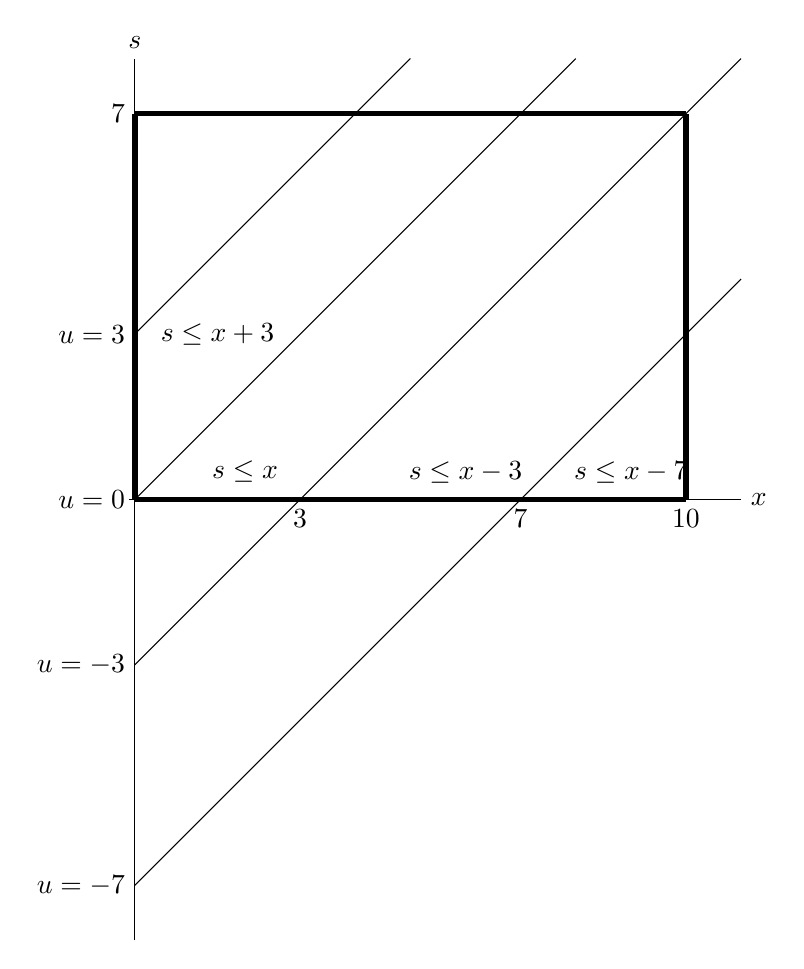
\begin{tikzpicture}[scale=0.7]
%\draw[[-{Triangle[open]},dotted] (0,10)--(8.5,10);
\draw (0,-8)--(0,8);
\node[right] at (11,0) {$x$};
\draw (-0.1,0)--(11,0);
\node[above] at (0,8) {$s$};
\draw[line width=0.7mm] (0,7)--(10,7);
\draw[line width=0.7mm] (10,0)--(10,7);
\draw[line width=0.7mm] (0,0)--(10,0);
\draw[line width=0.7mm] (0,0)--(0,7);
\node[below] at (10,0) {10};
\node[below] at (7,0) {7};
\node[below] at (3,0) {3};
\node[left] at (0,7) {7};
\draw (0,-7)--(11,4);
\node[left] at (0,-7) {$u=-7$};
\node at (9,0.5) {$s\leq x - 7$};
\draw (0,-3)--(11,8);
\node[left] at (0,-3) {$u=-3$};
\node at (6,0.5) {$s\leq x - 3$};
\draw (0,0)--(8,8);
\node[left] at (0,0) {$u=0$};
\node at (2,0.5) {$s\leq x$};
\draw (0,3)--(5,8);
\node[left] at (0,3) {$u=3$};
\node at (1.5,3) {$s\leq x+3$};
\end{tikzpicture}
\end{center}
%\caption{Computing the probability that $S-X\leq u$.}
%\label{fig:P_S_X}
%\end{figure}


It is clear that  the indicated rectangle has no overlap with the set of points $(x,s)$ such that $s\leq u + x$ for $u<-10$. (To see this, draw the line $s=x-10$ in the figure.) At $u=-10$, the overlap is a single point, at $(10,0)$. Thus, 
\begin{equation*}
\P{S-X \leq u}=0, \quad \text{for } u\leq -10.
\end{equation*}

For $u\in[-7, -3]$ we need to integrate over the triangle that results from cutting the line $s=x+u$ with the rectangle. The area is 
\begin{equation*}
70\, \P{S-X \leq u}= \frac{(10+u)^2}2, \quad \text{for } -7 \leq u\leq -3,
\end{equation*}
where we multiply with $70$ to get the normalization right. 

For $u\in[-3, 0]$, we integrate over a parallellogram with base $3+u$ and height $7$ plus the triangle below the line $s=x-3$. The area is 
\begin{equation*}
70\, \P{S-X \leq u}= (3+u)7 + \frac{(10-3)^2}2=7u + \frac{91}2, \quad \text{for } -3 \leq u\leq 0.
\end{equation*}

For $u\in[0, 7]$, we integrate over the trapezoid that results from intersecting the set $\{(x,s) : x \leq s \leq s + u\}$ and the rectangle plus the parallellogram plus the triangle below the line $s=x-3$. The area is 
\begin{equation*}
70\, \P{S-X \leq u}=  \frac{7^2}2 - \frac{(7-u)^2}{2} + 3\cdot 7 + \frac{49}2 = 7 u - \frac{u^2}2 + \frac{91}2, \quad \text{for } 0\leq u\leq 7.
\end{equation*}

Finally, for $u\geq 7$, the set $s\leq x+u$ covers the entire rectangle. Hence, 
\begin{equation*}
70\, \P{S-X \leq u}=  70, \quad \text{for } 7\leq u.
\end{equation*}

Given the amount of effort I had to put into getting this answer, I wanted to check it. So I went to  Wolframalpha (which is a great site for symbolic computations), and typed this: 
\begin{verbatim}
\int_{0}^{10} \int_0^7 Boole[s<= x + u]  ds dx,
\end{verbatim}
so, once you know \LaTeX\/ you can use Wolframalpha.  Wolframalpha turned it to 
\begin{verbatim}
Integrate[Boole[s <= u + x], {x, 0, 10}, {s, 0, 7}]
\end{verbatim}
If you fill this in at Wolframalpa, you'll get the results that we obtained above in seconds, rather than in one hour or so (depending on your proficiency with carry out integrals).
\end{solution}
\end{exercise}



\begin{exercise}
  A machine serves two types of jobs. The processing time of jobs of
  type $i$, $i=1,2$, is exponentially distributed with parameter
  $\mu_i$. The type $T$ of job is random and independent of anything
  else, and such that $\P{T=1} = p = 1-q = 1-\P{T=2}$. (An example
  is a desk serving men and women, both requiring different average
  service times, and $p$ is the probability that the customer in
  service is a man.)  Show that  the expected processing time  and  variance are given by
\begin{align*}
  \E X &= p \E{X_1}  + q \E{X_2} \\
\V X &= p \V{X_1} + q \V{X_2} + pq(\E{X_1} - \E{X_2})^2.
  \end{align*}
Interestingly, we see that even if $\V{X_1} = \V{X_2} = 0$, $\V X > 0$
if $\E{X_1} \neq \E{X_2}$. Bear this in mind; we will use these ideas
later when we discuss the effects of failures on the variance of
service times of jobs.
\begin{hint}
    Let $X$ be the processing (or service) time at the server, and
    $X_i$ the service time of a type $i$ job. Then, 
    \begin{equation*}
      X = \1{T=1} X_1 + \1{T=2} X_2,
    \end{equation*}
    where $\1{}$ is the indicator function, that is, $\1{A}=1$ if the
    event $A$ is true, and $\1{A}=0$ if $A$ is not true.   
\end{hint}
  \begin{solution}
With the hint, 
\begin{equation*}
  \begin{split}
  \E X 
&= \E{\1{T=1} X_1} + \E{\1{T=2} X_2} \\
&= \E{\1{T=1}} \E{ X_1} + \E{\1{T=2}} \E{X_2}, \text{ by the independence of $T$}, \\
&= \P{T=1} /\mu_1 + \P{T=2}/ \mu_2 \\
&= p /\mu_1 + q/ \mu_2 \\
&= p \E{X_1}  + q \E{X_2}.
  \end{split}
\end{equation*}
(The next derivation may seem a bit long, but the algebra is
standard. I include all steps so that you don't have to use pen and
paper yourself if you want to check the result.) Next, using that
\begin{equation*}
\1{T=1}\1{T=2} = 0 \text{ and } \1{T=1}^2 = \1{T=1},
\end{equation*}
we get
\begin{equation*}
  \begin{split}
  \V X 
&= \E{X^2} - (\E X)^2 \\
&= \E{\left(\1{T=1} X_1 + \1{T=2} X_2\right)^2} - \left(\frac{p}{\mu_1}+\frac{q}{\mu_2}\right)^2 \\
&= \E{\1{T=1} X_1^2 + \1{T=2} X_2^2} - \left(\frac{p}{\mu_1}+\frac{q}{\mu_2}\right)^2 \\ 
&= p \E{X_1^2} + q \E{X_2^2} - \left(\frac{p}{\mu_1}+\frac{q}{\mu_2}\right)^2 \\ 
&= p \V{X_1} + p (\E{X_1})^2 + q \V{X_2} + q(\E{ X_2})^2 - \left(\frac{p}{\mu_1}+\frac{q}{\mu_2}\right)^2 \\ 
&= p \V{X_1} + \frac{p}{\mu_1^2} + q \V{X_2} + \frac{q}{\mu_2^2} - \left(\frac{p}{\mu_1}+\frac{q}{\mu_2}\right)^2 \\ 
&= p \V{X_1} + q \V{X_2}
+ \frac{p}{\mu_1^2} + \frac{q}{\mu_2^2}
- \frac{p^2}{\mu_1^2}-\frac{q^2}{\mu_2^2}  -\frac{2pq}{\mu_1\mu_2}\\ 
&= p \V{X_1} + q \V{X_2}
+ \frac{p(1-p)}{\mu_1^2} + \frac{q(1-q)}{\mu_2^2}
-\frac{2pq}{\mu_1\mu_2}\\ 
&= p \V{X_1} + q \V{X_2}
+ \frac{pq}{\mu_1^2} + \frac{qp}{\mu_2^2}
-\frac{2pq}{\mu_1\mu_2}\\ 
&= p \V{X_1} + q \V{X_2}
+ pq(\E{X_1} - \E{X_2})^2.
\end{split}
\end{equation*}
\end{solution}
\end{exercise}


Let $B$ be a discrete random variable  such that $\P{B = k} = f(k)$, where $f(k)$ is a given set of
probabilities. We write
\begin{equation*}
  G(k) = \P{B>k} = \sum_{m=k+1}^\infty f(m),
\end{equation*}
for the \emph{survivor function} of $B$.  We can write this with an indicator function as
\begin{equation*}
  G(k) = \sum_{m=0}^\infty \1{m>k} f(m),
\end{equation*}
which makes the compution of certain expressions quite a bit easier. 

\begin{exercise}\label{ex:6}
 Use indicator functions to prove that $ \sum_{k=0}^\infty G(k) = \E B$.
    \begin{hint}
Write 
$\sum_{k=0}^\infty G(k) = \sum_{k=0}^\infty \sum_{m=k+1}^\infty \P{B=m}$, reverse the summations. Then realize that $\sum_{k=0}^\infty \1{k<m} = m$. 
You should be aware that this sort of problem is just a regular probability
  theory problem, nothing fancy. We use/adapt the tools you learned in
  calculus to carry out 2D integrals (or in this case 2D summations.)
    \end{hint}
\begin{solution}
\begin{align*}
\sum_{k=0}^\infty G(k) 
&= \sum_{k=0}^\infty \P{B>k} 
= \sum_{k=0}^\infty \sum_{m=k+1}^\infty \P{B=m}  \\
& = \sum_{k=0}^\infty \sum_{m=0}^\infty 1\{m>k\} \P{B=m} 
= \sum_{m=0}^\infty \sum_{k=0}^\infty 1 \{m>k\} \P{B=m} \\
&= \sum_{m=0}^\infty m\P{B=k} = \E B.
\end{align*}
In case you are interested in mathematical justifications: the
interchange of the two summations is allowed because the summands are
all positive. (Interchanging the order of summations or integration is
not allways allowed because the results can be different when part of
the integrand is negative. Check Fubini's theorem for more on this if
you are interested.)
\end{solution}
\end{exercise}

\begin{exercise}\label{ex:66}
 Use indicator functions to prove that
$\sum_{i=0}^\infty i G(i) =  \E{B^2}/2 - \E{B}/2.$
    \begin{hint}
$\sum_{i=0}^\infty i G(i) = \sum_{n=0}^\infty \P{B=n} \sum_{i=0}^\infty i 1\{n\geq i+1\}$,
and reverse the summations.
    \end{hint}
\begin{solution}
\begin{align*}
\sum_{i=0}^\infty i G(i)
&= \sum_{i=0}^\infty i \sum_{n=i+1}^\infty \P{B=n} = \sum_{n=0}^\infty \P{B=n} \sum_{i=0}^\infty i 1\{n\geq i+1\} \\
&= \sum_{n=0}^\infty \P{B=n} \sum_{i=0}^{n-1}i  = \sum_{n=0}^\infty \P{B=n} \frac{(n-1)n}{2} \\
&= \sum_{n=0}^\infty  \frac{n^2}{2} \P{B=n} - \frac{\E B}{2}
= \frac{\E B^2}2 - \frac{\E B}{2}.
\end{align*}
\end{solution}
\end{exercise}


Let $S$ be a continuous random variable $S$ with distribution function $F$.  We write 
\begin{equation*}
  \E{X} = \int_0^\infty x \d F(x)
\end{equation*}
for the expection of $X$. Here $\d F(x)$ acts as a shorthand for $f(x) \d x$ when $X$ has a density. \footnote{For the interested $\int x \d F(x)$ is a Lebesgue-Stieltjes integral with respect to the measure induced by the distribution function $F$.}

\begin{exercise}
 Use indicator functions to prove that 
$   \E S = \int_0^\infty x \d F  = \int_0^\infty G(y) \d y,$
where $G(x) = 1 - F(x)$. 
\begin{hint}
$\E S = \int_0^\infty x \d F  = \int_0^\infty \int_0^\infty 1_{y\leq x} \d y \d F(x)$.
\end{hint}
\begin{solution}
\begin{equation*}
  \begin{split}
    \E{S} &= \int_0^\infty x \d F  = \int_0^\infty \int_0^x \d y \d F(x) \\
    & = \int_0^\infty \int_0^\infty 1_{y\leq x} \d y \d F(x)   = \int_0^\infty \int_0^\infty 1_{y\leq x} \d F(x) \d y\\
    & = \int_0^\infty \int_y^\infty \d F(x) \d y = \int_0^\infty G(y) \d y
  \end{split}
\end{equation*}
\end{solution}
\end{exercise}

\begin{exercise}
 Use indicator functions to prove that for  a continuous random
    variable $S$ with distribution function $F$, 
$    \E{S^2} = \int_0^\infty x^2 \d F  = 2 \int_0^\infty y G(y) \d y,$
where $G(x) = 1 - F(x)$. 
\begin{hint}
$\int_0^\infty y G(y) \d y = \int_0^\infty y \int_0^\infty 1\{y\leq x\}f(x)\, \d x \d y$.
\end{hint}
\begin{solution}
  \begin{equation*}
    \begin{split}
\int_0^\infty y G(y) \d y 
&=  \int_0^\infty y \int_y^\infty f(x)\, \d x \d y =  \int_0^\infty y \int_0^\infty 1\{y\leq x\}f(x)\, \d x \d y\\
&=  \int_0^\infty f(x) \int_0^\infty y 1\{y \leq x\}\, \d x \d y
=  \int_0^\infty f(x) \int_0^x y\, \d x \d y\\
&=  \int_0^\infty f(x) \frac{x^2}2 \d x =\frac{\E S^2}2.
    \end{split}
  \end{equation*}
\end{solution}
\end{exercise}

\begin{exercise}
 Use integration by parts to show that for  a continuous random
    variable $S$ with distribution function $F$ and survivor function $G=1-F$, 
$\int_0^\infty y G(y) \d y = \E{S^2}/2.$
\begin{solution}
  \begin{equation}
      \int_0^\infty y G(y) \d y 
= \frac{y^2}2 G(y) \bigg|_0^\infty  - \int_0^\infty \frac{y^2}2 g(y)\d y = \int_0^\infty \frac{y^2}2 f(y)\d y = \frac{\E{S^2}}2,
  \end{equation}
  since $g(y) = G'(y) = - F'(y) = f(y)$.
\end{solution}
\end{exercise}

\begin{exercise}
  Use that $\E S = \int_0^\infty x \d F = \int_0^\infty G(y) \d y$ to
  check that  $\E S = \mu^{-1}$ if $F(x) = 1 - e^{-\mu x}$.
\begin{solution}
If $F(x) = 1 - e^{-\mu x}$, we obtain that 
\begin{equation*}
  \E S = \int_0^\infty e^{-\mu x} \d x =
  \mu^{-1}\int_0^\infty e^{-x} \d x = \mu^{-1}.
\end{equation*}
\end{solution}
\end{exercise}


\begin{comment}
\begin{exercise}
  Assume that the time $X$ to fail of a machine is uniformly
  distributed on the interval $[0,10]$. If the machine fails at time
  $t$, the cost to repair it is $h(t)$. What is the expected repair
  cost? 
  \begin{solution}
    Write for $F(x) = \P{X\leq x}$ and $f(x) = \d F(x)/\d x$ for the
    density of $F$.
    \begin{equation*}
      \begin{split}
\E{h(X)}
&= \int_0^{10} \E{h(X) \given X = x} \P{X\in \d x} \\
&= \int_0^{10} \E{h(x) \given X = x} \d F(x) \\
&= \int_0^{10} \E{h(x) \given X = x} F(\d x) \\
&= \int_0^{10} \E{h(x) \given X = x} f(x) \d x \\
&= \int_0^{10} h(x)\frac{\d x}{10}.
      \end{split}
    \end{equation*}
    Here we introduce some notation that is commonly used in the
    probabity literature to indicate the same conceptual idea, i.e,
    $\P{X\in \d x} = \d F(x) = F(\d x) = f(x) \d x$, where the last
    equality follows from the fact that $F$ has a density $f$
    everywhere on $[0,10]$. 

    The concept of conditional expectation is of fundamental
    importance in probability theory. Any \emph{good} probability book
    defines this concept as a random variable measurable with respect
    to some $\sigma$-algebra. In this course we will not deal with
    this elegant idea, due to lack of time. 
  \end{solution}
\end{exercise}
\end{comment}


\Closesolutionfile{hint}
\Closesolutionfile{ans}
\subsection*{Hints}
\input{hint}
\subsection*{Solutions}
\input{ans}

\clearpage  


%%% Local Variables:
%%% mode: latex
%%% TeX-master: "book"
%%% End:
